\section{LLM-based AI-Systems and Agents in General (RQ2)}
\label{sec:ai-agents}

The previous chapters examined remote meetings, facilitation, and existing GSS primarily from an application
perspective. In the case of the last, technical approaches were also described. To address RQ2,
typical patterns to LLM-based AI systems are also relevant, as well as the possibility of testing these
assumptions. However, this chapter does not claim to be exhaustive but serves primarily to clarify what the
author has focused on.

% ---------------------------------------------------------------------------------------------------------------------
\subsection{Agentic Systems vs. Programmatic Automation / Workflows}
\label{sec:agentic-systems-vs-programmatic-automation-workflows}

Huang explains that it is difficult to provide a correct and complete definition of the term “AI agent”
because our understanding of it and the technologies behind it are changing rapidly. \cite[p.
2]{huangAgenticAITheories2025}

In addition, there is a subjective impression that the term “AI agent” is used excessively and inconsistently
in the literature, which leads to a diffuse understanding of the concept. To narrow down the definition of
the term, this thesis attempts to approach the concept by distinguishing it from programmatic automation methods.

In this thesis, “programmatic process automation” refers to the rule-based automation of
workflows, in which defined conditions and structured decision-making logic are used to execute processes efficiently,
reliably, and reproducibly.

While traditional software executes predefined instructions, “AI agents possess the capacity to initiate
actions, make decisions, and pursue goals without constant human intervention” \cite[p. 2]{huangAgenticAITheories2025}

Thus, AI agents have a higher degree of autonomy in this context.

Anthropic uses the following definition for LLM-based workflows and agents:

\begin{quote}
  "Workflows are systems where LLMs and tools are orchestrated through predefined code paths.
  Agents, on the other hand, are systems where LLMs dynamically direct their own processes and tool usage,
  maintaining control over how they accomplish tasks." \cite{anthropicBuildingEffectiveAI}
\end{quote}

Existing papers, such as the study by Houtti et al. or by Liu et al.
\cite{liuProactiveConversationalAgents2025}, also refer to an AI agent, for example, although it is
questionable whether these can be classified as AI agents according to Antroplic’s definition or whether they
are rather LLM-based workflows.
The system developed by Houtti et al. does not use any LLMs. The authors themselves state that they used a
rule-based prototype system to perform better testing. \cite{houttiObserveAskIntervene2025} Nevertheless,
they refer to it as an AI agent.

For the purposes of this thesis, it should therefore suffice for now to provide a rough classification of
whether the developed system is more agent-based or workflow-based. In this thesis, therefore mostly uses the
general term “AI system” for certain conclusions or system descriptions. When other systems are cited and the
authors use the term “AI agent,” this term has been adopted.

A description of the actual system can be found in the section on system architecture.

% ---------------------------------------------------------------------------------------------------------------------
\subsection{Prompt Engineering and Context Engineering}
\label{sec:context-engineering}

In general, context engineering refers to the design, organization, and management of context-sensitive information,
so that machines act in accordance with human intent. \cite[p. 3]{huaContextEngineering202025}

Although context engineering already played a role in early human-computer interaction frameworks
\cite[p. 1]{huaContextEngineering202025}, research has recently placed greater emphasis on this field due to
the growing challenges in
human-agent interaction (HAI).

In their meta-study \cite{meiSurveyContextEngineering2025}, Mei et al. (2025) analyzed over 1,400 research
papers on the topic of context engineering for LLMs. According to the authors, LLMs have evolved from simple
systems that merely follow instructions (so-called prompt engineering) into central inference modules. In the
process, the design and management of information content has developed into a discipline in its own right
(context engineering) \cite{meiSurveyContextEngineering2025}

For LLM-based systems, context engineering can be defined as follows::

\begin{quote}
  "Context engineering is the practice of deliberately structuring and optimizing the information passed to an
  LLM or Agent to produce more accurate and relevant outputs." \cite[00:34]{ibmtechnologyWhatContextEngineering2026}
\end{quote}

Context engineering thus goes beyond traditional prompt engineering and encompasses advanced methods such as
retrieval-augmented generation (RAG), memory systems, tool-integrated reasoning, and multi-agent systems
(see Mei et al., 2025). \cite[p. 12-26]{meiSurveyContextEngineering2025}

\begin{figure}[htbp]
  \centering
  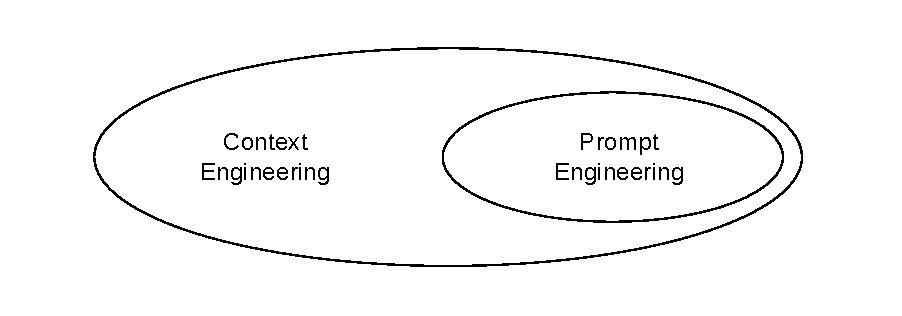
\includegraphics[width=0.9\textwidth]{assets/figures/02/venn-context-and-prompt-engineering.pdf}
  \caption{Venn-Diagram: Prompt Engineering as a subset of Context Engineering
  \figsource{Own illustration, created with draw.io.}}
  \label{fig:venn-diagram-prompt-engineering-context-engineering}
\end{figure}

Although various methods of context engineering are discussed in the literature, Mei et al.
critically point out that current practice operates without a unified theoretical foundation. Such a
foundation would be necessary to link the various techniques together and
derive principle-based design guidelines. This research gap is further exacerbated by the lack of
mathematical frameworks that would make it possible to characterize optimal design principles for context
engineering in complex systems. This is related to the lack of methods
for determining the optimal context composition. \cite[p. 51]{meiSurveyContextEngineering2025}

%%%%%%%
% ---------------------------------------------------------------------------------------------------------------------
\FloatBarrier
\subsection{Building blocks for LLM-based Workflows and Agents}
\label{sec:ai-agent-building-blocks}

In order to develop the AI agent described later, it was first necessary to examine the fundamental building
blocks of AI agents.
Anthropic has published a blog post on this topic, \cite{anthropicBuildingEffectiveAI}, which summarizes
these fundamental building blocks from their perspective and serves as the primary basis for this chapter. We
first examined all currently common patterns, even though not all of them were ultimately used in the actual system.

\newpage

\textbf{Prompt chaining}

\begin{figure}[H]
  \centering
  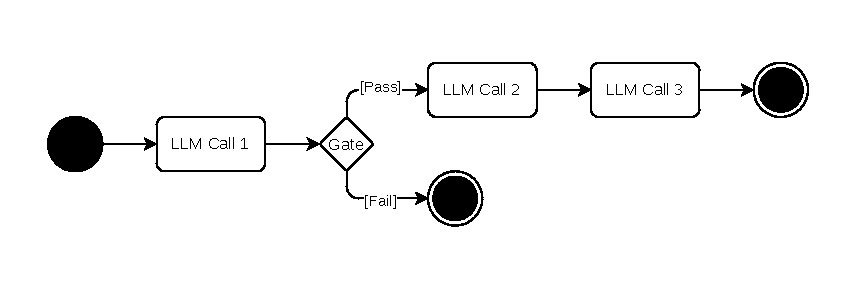
\includegraphics[width=0.9\textwidth]{assets/figures/02/prompt-chaining.pdf}
  \caption{AI-Building-Block:Prompt chaining: A complex task is decomposed into sequential LLM calls
    \figsource{Own illustration based on "Building Effective AI Agents by
  Anthropic"\cite{anthropicBuildingEffectiveAI}, created with draw.io.}}
  \label{fig:prompt-chaining}
\end{figure}

In prompt chaining, a complex task is broken down into a sequential series of substeps. Each step is
described by a prompt and an LLM call, which uses the result of the previous step as context for the next step.
Programmatic checks can be inserted in between. \cite{anthropicBuildingEffectiveAI}

\textbf{Routing}

\begin{figure}[H]
  \centering
  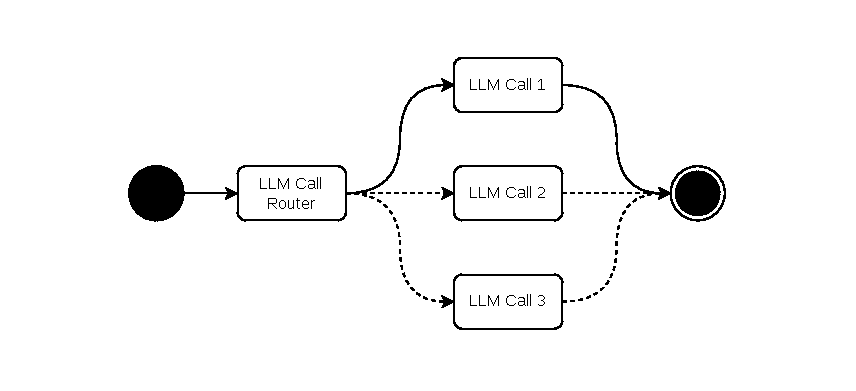
\includegraphics[width=0.9\textwidth]{assets/figures/02/routing.pdf}
  \caption{AI-Building-Block:Routing: A complex task is decomposed into subtasks and routed to specialized systems
    \figsource{Own illustration based on "Building Effective AI Agents by
  Anthropic"\cite{anthropicBuildingEffectiveAI}, created with draw.io.}}
  \label{fig:routing}
\end{figure}

During routing, tasks are classified and forwarded to subsystems that specialize in solving that category of
tasks. This results in a clear separation of responsibilities, which
is particularly well-suited when complex tasks can be divided into clearly definable categories and
processed by specialized LLMs, other AI models, or algorithms. \cite{anthropicBuildingEffectiveAI}

\textbf{Parallelization}

\begin{figure}[H]
  \centering
  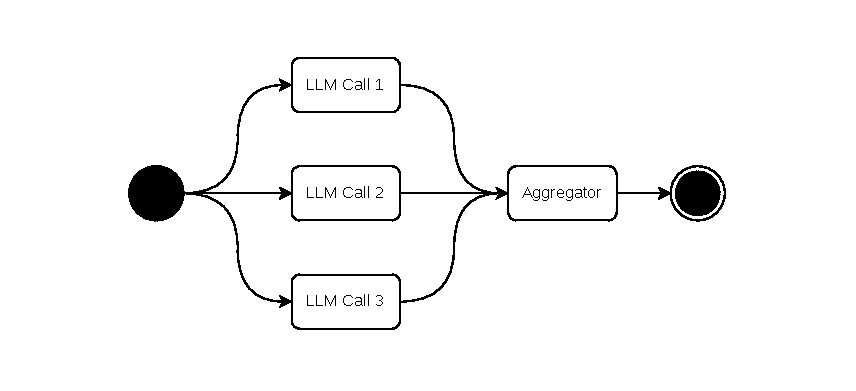
\includegraphics[width=0.9\textwidth]{assets/figures/02/parallelization.pdf}
  \caption{AI-Building-Block: Parallelization: Multiple tasks are processed in parallel and the results are
    aggregated programatically
    \figsource{Own illustration based on "Building Effective AI Agents by
  Anthropic"\cite{anthropicBuildingEffectiveAI}, created with draw.io.}}
  \label{fig:parallelization}
\end{figure}

In the parallelization workflow, multiple tasks are processed simultaneously, and the results
are aggregated programmatically. Typical use cases arise when tasks can be broken down into independent subtasks
or when multiple perspectives are required to achieve a more reliable result
(e.g. voting). For complex tasks with multiple aspects, LLMs achieve better results
when each aspect is addressed separately using a specialized prompt. \cite{anthropicBuildingEffectiveAI}

\textbf{Orchestrator-workers}

\begin{figure}[H]
  \centering
  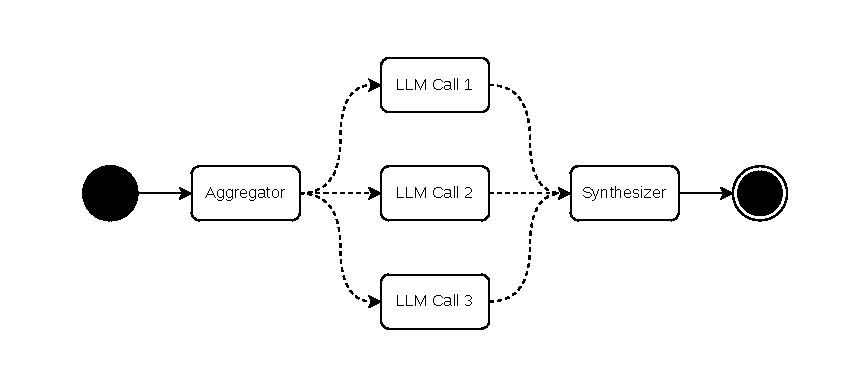
\includegraphics[width=0.9\textwidth]{assets/figures/02/orchestrator-workers.pdf}
  \caption{AI-Building-Block: Orchestrator-workers: A central LLM decomposes a main task dynamically into
    subtasks and delegates
    them to a variable number of worker LLMs
    \figsource{Own illustration based on "Building Effective AI Agents by
  Anthropic"\cite{anthropicBuildingEffectiveAI}, created with draw.io.}}
  \label{fig:orchestrator-workers}
\end{figure}

The Orchestrator-Worker workflow is similar to the parallelization workflow, but differs in that
it is used when the required subtasks are not known in advance. A central LLM dynamically breaks down
the main task into subtasks and delegates them to any number of worker LLMs,
whose results are then aggregated. \cite{anthropicBuildingEffectiveAI}

\textbf{Evaluator-optimizer}

\begin{figure}[H]
  \centering
  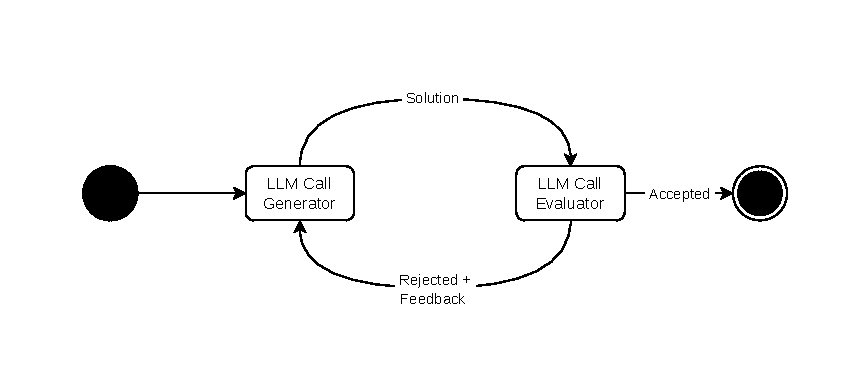
\includegraphics[width=0.9\textwidth]{assets/figures/02/evaluator-optimizer.pdf}
  \caption{AI-Building-Block: Evaluator-optimizer: A LLM generates answers, while another evaluates and
    optimizes them through feedback
    \figsource{Own illustration based on "Building Effective AI Agents by
  Anthropic"\cite{anthropicBuildingEffectiveAI}, created with draw.io.}}
  \label{fig:evaluator-optimizer}
\end{figure}

The evaluator-optimizer workflow uses a feedback loop in which one LLM generates responses while another
evaluates them and attempts to optimize them through feedback. This approach is particularly effective when
clear evaluation criteria are in place and iterative improvements are measurable. \cite{anthropicBuildingEffectiveAI}

% ---------------------------------------------------------------------------------------------------------------------
\subsection{Evaluating and Testing of AI-Systems}
\label{sec:evaluating-ai-systems}

Due to the probabilistic nature of AI-based systems, testing
AI-based systems differs fundamentally from conventional testing methods.

The International Software Testing Qualifications Board (ISTQB®) therefore suggests that this probabilistic
nature would require statistical testing methods. \cite[p. 39]{istqbrISTQBCertifiedTester}

An additional challenge is that some AI systems are not only static but also
adaptive, and can therefore continuously adjust themselves \cite[p.~39]{istqbrISTQBCertifiedTester}.

These adjustments can occur on at least two levels::
\begin{itemize}
  \item \textbf{Context-Based Adaptation:} Within the application, the AI system can dynamically adapt to
    changing conditions or the diverse possibilities offered by the
    context available at that moment.
  \item \textbf{Model-Based Adaptation:} Regardless of the specific context of the use case, the
    underlying AI models may change on their own, for example through the use of self-learning algorithms. When
    integrating external large language models (LLMs), the provider may make modifications to the model
    that are not immediately apparent to the user.
\end{itemize}
Defining a test oracle that is, specifying the expected outputs for specific input values for the system
under test is therefore extremely difficult or even impossible in complex AI systems
\cite[p.~39]{istqbrISTQBCertifiedTester}.

In a live meeting scenario, context-based adaptation is particularly relevant. In any given meeting, there
may be a variety of participants working on different topics, which makes the context in which the AI system
operates highly variable.

Mohammadi et al. \cite[p. 1]{mohammadiEvaluationBenchmarkingLLM2025} also point out that evaluating and
testing LLM-based agents is a complex and still under-researched field, particularly because
agents often operate in a more dynamic and interactive context.
They therefore describe the testing of LLM agents as an interplay of the various perspectives of natural
language processing (NLP), human-computer interaction (HCI), and software engineering.

\phantomsection\label{sec:code-based-testing}
Code-based methods aim to evaluate the performance of AI systems using explicit
program code, defined rules, and test cases with assertions. This involves verifying whether the
actions performed exactly meet specified criteria. \cite[p. 7]{mohammadiEvaluationBenchmarkingLLM2025}

For this purpose, for example, possible states that the system goes through can be modeled and analyzed using
trajectory comparisons. However, existing benchmarking methods such as AgentBoard
\cite{maAgentBoardAnalyticalEvaluation2024} are often
general in nature and only partially suitable for domain-specific use cases.

Code-based methods reach their limits, particularly with open-ended or qualitative responses, as well as with
creative problems where correctness
can be evaluated subjectively
\cite[p.~7]{mohammadiEvaluationBenchmarkingLLM2025}.

\phantomsection\label{sec:llm-as-a-judge}
The “LLM-as-a-Judge” approach leverages the reasoning capabilities of LLMs to evaluate agents' responses based on
qualitative criteria. In this process, the responses are analyzed based on
the evaluation metrics specified in the instructions. \cite[p.~7]{mohammadiEvaluationBenchmarkingLLM2025}.

The authors Zheng et al. \cite[p. 4]{zhengJudgingLLMasaJudgeMTBench2023} propose three variants of the
LLM-as-a-Judge approach, which can be applied individually or in combination:
\begin{itemize}
  \item Pairwise Comparison: An LLM compares two answers to a question and decides which is better or whether
    there is a tie.
  \item Single Answer Grading: An LLM evaluates a single answer directly using a scale or a set of criteria.
  \item Reference-Guided Grading: An LLM evaluates an answer by comparing it to a given
    reference solution, e.g., for math problems.
\end{itemize}

The appendix to the paper “Judging LLM-as-a-Judge with MT-Bench and Chatbot Arena” contains the corresponding
prompts that can be used for the various variants of the LLM-as-a-Judge approach
\cite{zhengJudgingLLMasaJudgeMTBench2023}.

According to Mohammadi et al., however, human-in-the-loop evaluation is still considered the gold standard, in which
people (such as in user studies, expert audits, or through crowdworkers) annotate or
evaluate the outputs \cite[p.~7]{mohammadiEvaluationBenchmarkingLLM2025}. However, this approach is often
difficult to scale and involves significant effort and costs.

A widely used approach is Evaluation-Driven Development (EDD), in which AI-based systems and agents
are continuously evaluated during the development phase to detect deviations and identify new use cases
\cite[p.~6]{mohammadiEvaluationBenchmarkingLLM2025}.